\chapter{SR Sensível ao Tempo}

\section{Algoritmo Proposto}

O algoritmo de recomendação proposto nesse trabalho combina a Abordagem Baseada em Conteúdo tradicional com o uso do
contexto temporal através da categoria \textit{Decay} (ver seção \ref{section:decay}).

O cálculo da relevância de um determinado item $i$ para um usuário $u$ no algoritmo proposto está formalizada na Equação
\ref{eq:relevancia-proposta}.

\begin{equation}
  F(u,i) = S(u,i) \cdot R(I_{u,i}) + A(i)
  \label{eq:relevancia-proposta}
\end{equation}

Onde: $F$ é a função que calcula a relevância de um item $i$ para um usuário $u$; $S$ é a função de similaridade entre
o perfil do usuário $u$ (representado através de conjunto de palavras-chave dos itens acessados) e o item $i$
(representado pelo conjunto de palavras-chave que o caracterizam); $R$ é o maior valor de recência dos itens do conjunto
$I_{u,i}$ (itens acessados pelo usuário $u$ e com alguma similaridade com o item $i$); $A$ é uma função que retorna $1$
se o item $i$ nunca foi acessado pelo usuário u e $0$ se o item já foi acessado.

A função $S$ de similaridade entre o usuário $u$ e o item $i$ é calculada utilizando a fórmula do cosseno (ver Seção
\ref{subsection:baseada-em-conteudo}). A função de recência $R$, responsável pelo \textit{Decay}, estéa definida na Equação
\ref{eq:recencia-proposta}.

\begin{equation}
  R(I_{u,i}) = \max_{\{j \in I_{u,i}\}}{\frac{x_j}{\left| I_u \right|}}
  \label{eq:recencia-proposta}
\end{equation}

Onde: $x_j$ é a posição do item j na lista de itens acessados pelo usuário $u$ ordenada de forma crescente pelo
\textit{timestamp} do acesso; e $\left| I_u \right|$ é a quantidade de itens acessados pelo usuário $u$. Essa fórmula considera
que mais de um item acessado pelo usuário pode ser similar ao item $i$, por isso a fórmula retorna a maior recência de
todos os itens presentes no perfil do usuário que são similares a $i$. A seguir temos um exemplo do uso da fórmula da
recência de um item, que pode ser estendida para o uso com vários itens e aplicada a função $max$ como descrito na
fórmula acima.

Suponha que um usuário $u$ acessou três itens diferentes nos seguintes \textit{timestamps} (em \textit{epoch}): Item A acessado $1503670382$;
Item B acessado em $1500027182$; Item C acessado em $1508051582$. Ao ordenar esses itens pelo \textit{timestamp}, em ordem
crescente, temos: (1) Item B, (2) Item A, (3) Item C. As equações \ref{eq:recencia-item-a}, \ref{eq:recencia-item-b} e
\ref{eq:recencia-item-c} apresentam o resultado do cálculo de recência para cada um dos itens:

\begin{equation}
  R(A) = \frac{2}{3} = 0.\overline{6}
  \label{eq:recencia-item-a}
\end{equation}

\begin{equation}
  R(B) = \frac{1}{3} = 0.\overline{3}
  \label{eq:recencia-item-b}
\end{equation}

\begin{equation}
  R(C) = \frac{3}{3} = 1.0
  \label{eq:recencia-item-c}
\end{equation}

\section{Discussão Sobre o Algoritmo Proposto}

Um ponto negativo da Filtragem Colaborativa é a necessidade de uma comunidade de usuários ativa, que nem sempre é
possível em um ambiente educacional onde as turmas muitas vezes são menores (entre 10 e 100 alunos). A Abordagem Baseada
em Conteúdo é considerada para o SR porque essa abordagem permite a recomendação em um sistema que não possui uma
comunidade ativa e supre as necessidades desse domínio.

Os SRs Sensíveis ao Tempo tem uma vantagem em relação à outros SRs Sensíveis ao Contexto por a informação temporal ser
mais simples de capturar e manipular que outras informações contextuais, e.g., localização. Além disso, esses tipos de
algoritmos estão sendo explorados em outros domínios de aplicação, como pode ser visto nos 88 artigos analisados no
Mapeamento Sistemático realizado \cite{de2017time}, e demonstraram bons resultados. Por isso, esse trabalho busca
aplicar o contexto temporal no algoritmo de recomendação na área educacional (na qual foram encontrados apenas quatro
trabalhos) e avaliar os resultados.

A escolha do \textit{Decay} se justifica como forma de resolver uma das grandes desvantagens da abordagem Baseada em Conteúdo: a
Superespecialização. Na abordagem Baseada em Conteúdo as recomendações seriam geradas levando em conta todos os itens
acessados pelo usuário igualitariamente. Enquanto ao aplicar o \textit{Decay}, os itens acessados mais recentemente possuem um
grau de importância maior para o algoritmo do que itens acessados anteriormente. Dessa forma, mesmo que o usuário
acessou muitos materiais sobre determinado assunto, ao começar a acessar materiais sobre outro assunto o algoritmo de
recomendação consegue rapidamente se adaptar e gerar recomendações sobre esse novo conteúdo.

Um cenário que justifica o uso do \textit{Decay} seria: o aluno Pedro está matriculado em uma disciplina de Estrutura de Dados
que possui quatro tópicos, sendo eles Pilhas, Filas, Listas e Árvores. Nessa disciplina, para cada um dos conteúdos é
aplicada uma prova para avaliar os conhecimentos dos alunos. Até o momento da primeira prova sobre o conteúdo de Pilhas,
Pedro acessou apenas materiais relacionados a Pilhas. O algoritmo de recomendação utilizando a abordagem Baseada em
Conteúdo recomenda para Pedro apenas materiais relacionados a Pilhas. Após a primeira prova, Pedro começa a acessar
materiais relacionados a Filas, o segundo tópico da disciplina. Em uma abordagem Baseada em Conteúdo tradicional as
recomendações continuariam sendo sobre o conteúdo de Pilhas por um bom tempo, pois o perfil de Pedro seria em grande
parte composto por materiais acessados sobre esse assunto. Porém, com o uso do \textit{Decay}, no momento em que Pedro começar a
acessar materiais sobre Filas o algoritmo de recomendação dará um peso maior para esses materiais (sem ignorar os itens
acessados anteriormente) e em pouco tempo Pedro já estará recebendo recomendações sobre o novo tópico estudado. Da mesma
forma, se Pedro voltar a acessar conteúdos anteriores para relembrar algum conceito, o SR também perceberá isso e
recomendará itens relacionados ao primeiro conteúdo novamente.

O algoritmo proposto nesse trabalho considera o decaimento no peso dos itens do perfil do usuário em função da posição
do item na sequência de materiais acessados, como mostrado anteriormente, e não na quantidade de tempo passada em
segundos como feito na maioria dos trabalhos relacionados mostrados no Capítulo \ref{chapter:trabalhos-relacionados}. Isso é uma vantagem, pois no domínio
educacional o passar do tempo não é tão relevante quanto em outros domínios, como na recomendação de \textit{Web Services} por
exemplo.

Os alunos em um ambiente educacional podem ter ritmos de estudo diferentes e, por isso, é assumido nesse trabalho que faz
mais sentido analisar quantos itens foram acessados desde do acesso de determinado material do que o tempo passado desde
a interação. Dessa forma, nesse algoritmo não faz diferença se o usuário acessou todos os itens do seu perfil em um
único dia, se ele acessou metade do materiais na primeira semana do curso e a outra metade na última semana ou se ele
acessou alguns materiais todos os dias durante o curso.

Além disso, no algoritmo proposto nesse trabalho não é necessário definir um fator de decaimento como nos trabalhos
relacionados apresentados no Capítulo \ref{chapter:trabalhos-relacionados}. Ao considerar um parâmetro como fator de decaimento seria necessário considerar
que cada aluno tem um estilo de aprendizagem diferente e o decaimento para um aluno poderia ser diferente do decaimento
para outros alunos. E não foram encontrados trabalhos que mostrem um modelo para calcular o fator de decaimento de forma
personalizada para cada usuário. Em geral, os autores utilizam o fator de decaimento escolhido de forma empírica e
aplicam o mesmo fator para todos os usuários.

\section{Descrição do Ambiente AdaptWeb\textsuperscript{\textregistered}}

O algoritmo proposto será incorporado ao ambiente AdaptWeb\textsuperscript{\textregistered}. O
AdaptWeb\textsuperscript{\textregistered} (Ambiente de Ensino-Aprendizagem Adaptativo na Web) é um sistema open source
que consiste em um AVA capaz de adaptar o conteúdo, a apresentação e a navegação em determinado curso às características
e preferências do aluno \cite{gasparini2009adaptweb}. A próxima seção apresenta a Estrutura Geral do
AdaptWeb\textsuperscript{\textregistered}.

\subsection{Estrutura do AdaptWeb\textsuperscript{\textregistered}}

A estrutura do AdaptWeb\textsuperscript{\textregistered} é composta por quatro módulos: (1) o módulo de autoria; (2) o
módulo de armazenamento em XML (Extensible Markup Language); (3) o módulo de adaptação do conteúdo baseado no modelo do
usuário e (4) o módulo de interface adaptativa \cite{gasparini2003interface}, conforme pode ser visto na Figura
\ref{fig:adaptweb-arquitetura}.

O módulo de autoria (1) consiste na organização do conteúdo instrucional a ser disponibilizado para o aluno, sendo que
este conteúdo pode ter arquivos classificados como conceito, exemplos, exercícios e materiais complementares
\cite{gasparini2003interface}. Ao criar um conteúdo no sistema, o autor pode definir para quais cursos e disciplinas
deseja que o conteúdo ou arquivo esteja disponível. Isto significa que um aluno de um Curso X e de outro Curso Y,
matriculados em uma mesma disciplina, podem ter conteúdos distintos, conforme definido pelo professor. Por exemplo, a
disciplina de Cálculo I pode ser oferecida para os cursos de Ciência da Computação e Engenharia Elétrica e sua
abrangência e profundidade pode ser distinta para cada curso.

\begin{figure}[htb]
  \caption{\label{fig:adaptweb-arquitetura}Estrutura do AdaptWeb\textsuperscript{\textregistered}}
  \begin{center}
      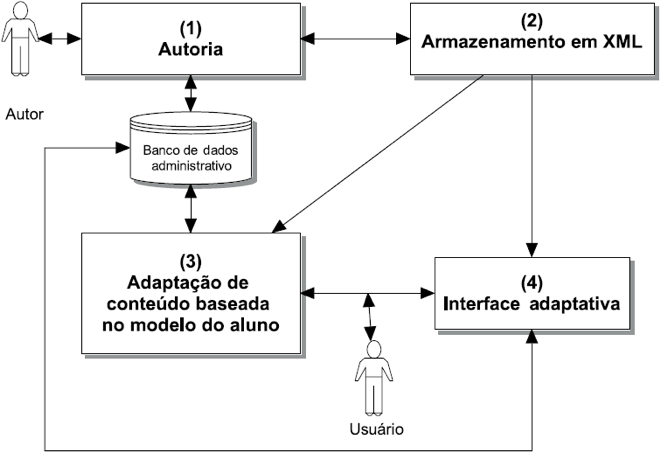
\includegraphics[scale=1.0]{./Figuras/adaptweb-arquitetura.png}
  \end{center}
  \legend{Fonte: \citeonline{gasparini2003interface}}
\end{figure}

O módulo de armazenamento em XML (2) é responsável por organizar os conteúdos e arquivos disponibilizados pelo autor em
um arquivo XML \cite{gasparini2003interface}. É utilizada a representação através de XML devido à sua alta
flexibilidade, oferecendo a estruturação dos documentos de forma independente da apresentação.

O módulo de adaptação do conteúdo baseado no modelo do aluno (3) é responsável por adaptar o conteúdo da disciplina
para cada curso. Por fim, o módulo de interface adaptativa (4) é responsável pela adaptação da navegação e da
apresentação da interface do ambiente de acordo com o curso, preferências do modo de navegação (modo tutorial ou livre)
e o conhecimento do usuário \cite{gasparini2003interface}.

\subsection{Sistema de Recomendação Presente no Ambiente}

O ambiente AdaptWeb\textsuperscript{\textregistered} possui um SR que foi desenvolvido em \citeonline{de2015sistema}. Em \citeonline{de2015sistema}
foi decidido que os OAs que o SR recomendaria são uma nova categoria de materiais da disciplina, não existente
originalmente no AdaptWeb\textsuperscript{\textregistered}, chamada "Links de Apoio", na qual o professor pode adicionar apenas links externos ao ambiente.

Para realizar a recomendação no AdaptWeb\textsuperscript{\textregistered}, o SR considera o último material complementar
que o aluno acessou, como também a lista de todos os materiais complementares acessados. Isto é feito porque se supõe
que, no contexto de um AVA, devem se considerar os interesses de curto e longo prazo do usuário \cite{xiang2010temporal}.

Na Figura \ref{fig:adaptweb-notificacao-recomendacao} pode ser observada a apresentação das recomendações para o aluno
através de uma notificação (destacada na Figura) proposta em \citeonline{de2015sistema}.

\begin{figure}[htb]
  \caption{\label{fig:adaptweb-notificacao-recomendacao}Interface do SR: Notificação de Link Recomendado}
  \begin{center}
      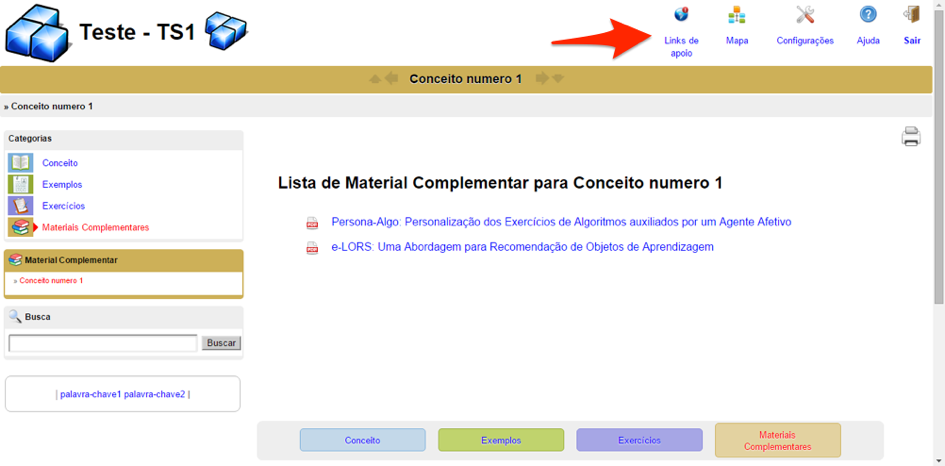
\includegraphics[scale=1.0]{./Figuras/adaptweb-notificacao-recomendacao.png}
  \end{center}
  \legend{Fonte: \citeonline{de2015sistema}}
\end{figure}

Ao clicar na notificação (indicada pela seta), é aberta uma janela pop-up com os links recomendados para aquele aluno.
Neste momento aparece o Título do Material e a Descrição, informados pelo professor. Além disso, é possível que o aluno
avalie o material, com uma nota de 1 a 5, e reporte links quebrados. A Figura 4 mostra a interface contendo as
recomendações realizadas em certo momento da interação do usuário.

\begin{figure}[htb]
  \caption{\label{fig:adaptweb-itens-recomendacao}Interface da Recomendação para o Aluno}
  \begin{center}
      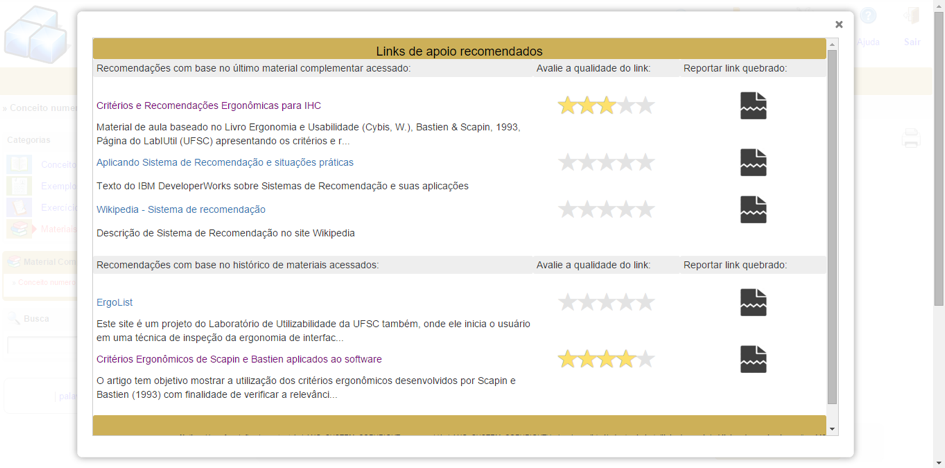
\includegraphics[scale=1.0]{./Figuras/adaptweb-itens-recomendacao.png}
  \end{center}
  \legend{Fonte: \citeonline{de2015sistema}}
\end{figure}

Em \citeonline{de2017sistema} foi feito um estudo com os dados de log gerados pela ferramenta de Learning Analytics
presente no ambiente. Nesse estudo foi possível observar que, dentro de um minicurso de algoritmos realizado, as
recomendações não foram percebidas pelos usuários. Dos 99 alunos ativos no minicurso, apenas 18 acessaram pelo menos
uma vez a área de recomendações. Além disso, dos 27.116 registros de páginas acessadas no ambiente, apenas 30 estão
relacionados ao SR \cite{de2017sistema}.

Por isso, nesse trabalho será considerado não só o algoritmo de recomendação, mas também uma forma mais eficiente de
apresentar essas recomendações. Isso porque não adianta o algoritmo de recomendação ser eficiente sendo que os alunos
nem sabem da existência dessa ferramenta. Na seção a seguir será apresentada a proposta de apresentação das
recomendações de forma a garantir que as recomendações chegem aos alunos.

\section{Apresentação das Recomendações}

Como mostrado anteriormente, o SR existente no AdaptWeb\textsuperscript{\textregistered} não é facilmente acessável pelos
alunos. A primeira decisão do presente trabalho foi mover as recomendações para a área principal do ambiente do aluno.
Dessa forma, se o SR possuir itens para recomendar para o usuário esses itens aparecem logo abaixo do conteúdo que ele estiver
visualizando no momento, independente se o aluno esteja na tela de Conceito, Exercícios, Exemplos ou Materiais Complementares.
Na Figura \ref{fig:adaptweb-proposta-recomendacao} pode-se observar os itens recomendados.

\begin{figure}[htb]
  \caption{\label{fig:adaptweb-proposta-recomendacao}Proposta de Interface de Recomendação}
  \begin{center}
      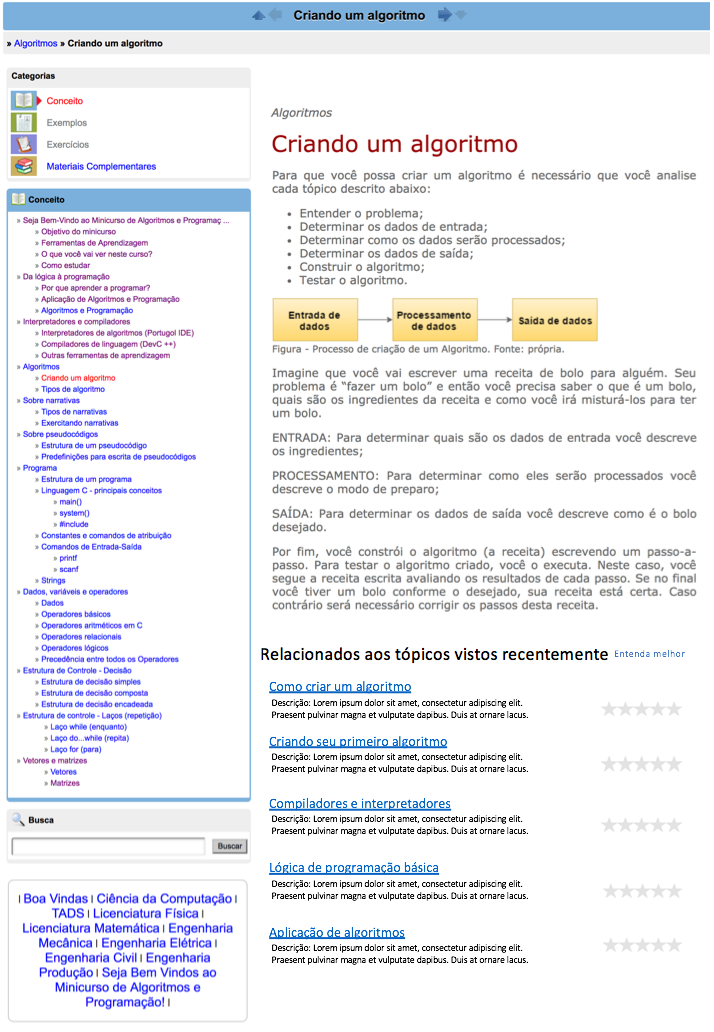
\includegraphics[scale=1.0]{./Figuras/recomendacoes_v2.png}
  \end{center}
  \legend{Fonte: O autor.}
\end{figure}

As principais informações dos links recomendados continuam sendo as mesmas que a versão anterior do SR: Link, Nome do Link,
Descrição e a possibilidade de avaliar o item com notas de 1 a 5. \citeonline{pu2012evaluating} afirmam que enquanto
recomendar um item apenas é pouco, recomendar mais do que cinco itens aumenta a dificuldade de escolhar do usuário. Por isso,
a quantidade máxima de itens recomendadas para o usuário em cada recomendação é de cinco itens.

Para cumprir o requisito de Explicação das recomendações citada por \citeonline{pu2012evaluating}, foi adicionado um
botão de "Entenda melhor" que tem por objetivo explicar ao usuário como a lista de itens foi gerada. Ao entender o
funcionamento do algoritmo de recomendação o usuário tem a possibilidade aprimorar o seu perfil para personalizar as
recomendações recebidas. Na Figura \ref{fig:adaptweb-proposta-explicacao} está a explicação da recomendação mostrada para o aluno.

\begin{figure}[htb]
  \caption{\label{fig:adaptweb-proposta-explicacao}Explicação da recomendação}
  \begin{center}
      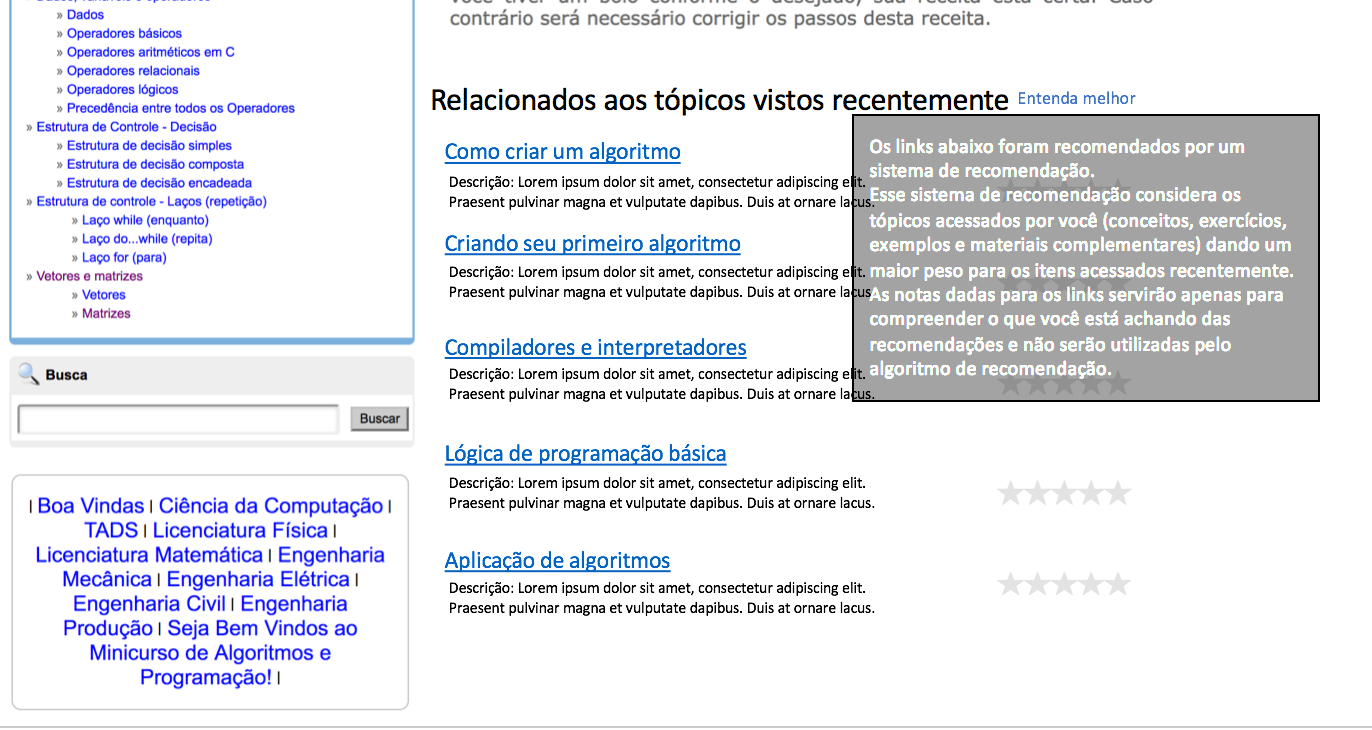
\includegraphics[scale=0.6]{./Figuras/explicacoes_v2.png}
  \end{center}
  \legend{Fonte: O autor.}
\end{figure}

\section{Considerações sobre o capítulo}
